% Compile with pdfLaTeX.
% Landscape version corresponding to the revised portrait template.
% Font matching is intentionally relaxed for this version.

\documentclass[a4paper,landscape]{article}

% Scroll down to line 74

% Minimal external packages:
\usepackage[a4paper,landscape,left=18mm,right=18mm,top=18mm,bottom=18mm]{geometry}
\usepackage{graphicx}
\usepackage{xcolor}
\usepackage{lipsum}
\usepackage{array}
\usepackage[T1]{fontenc}
\usepackage[sfdefault]{roboto}
\usepackage[
    colorlinks=true,
    urlcolor=blue,
    linkcolor=black,
    citecolor=blue
]{hyperref}

\pagestyle{empty}
\setlength{\parindent}{0pt}
\setlength{\parskip}{0pt}
\setlength{\tabcolsep}{0pt}
\definecolor{topicblue}{HTML}{2F5597}

% Lengths - specifications for template fonts, appearance
\newlength{\HeaderSize}
\setlength{\HeaderSize}{24pt}
\newlength{\HeaderSizeBaseline}
\setlength{\HeaderSizeBaseline}{28.8pt}

\newlength{\SectionSize}
\setlength{\SectionSize}{16pt}
\newlength{\SectionSizeBaseline}
\setlength{\SectionSizeBaseline}{1.2\SectionSize}

\newlength{\TextSize}
\setlength{\TextSize}{14pt}
\newlength{\TextSizeBaseline}
\setlength{\TextSizeBaseline}{1.3\TextSize}

\newlength{\CaptionSize}
\setlength{\CaptionSize}{12pt}
\newlength{\CaptionSizeBaseline}
\setlength{\CaptionSizeBaseline}{1.2\CaptionSize}

\newlength{\RefSize}
\setlength{\RefSize}{12pt}
\newlength{\RefSizeBaseline}
\setlength{\RefSizeBaseline}{1.4\RefSize}

\newlength{\vskipHeader}
\setlength{\vskipHeader}{8.0mm}
\newlength{\vskipSection}
\setlength{\vskipSection}{4.0mm}
\newlength{\vskipText}
\setlength{\vskipText}{2.0mm}
\newlength{\vskipImage}
\setlength{\vskipImage}{16.0mm}

% Landscape geometry.
% The left panel is square; the right panel uses the remaining width.
\newlength{\LeftPanel}
\setlength{\LeftPanel}{164mm}
\newlength{\PanelGap}
\setlength{\PanelGap}{18mm}
\newlength{\RightPanel}
\setlength{\RightPanel}{79mm}

% Do not change anything above this line!

\begin{document}
\noindent
\begin{tabular}{@{}p{\LeftPanel}@{\hspace{\PanelGap}}p{\RightPanel}@{}}

% ======================= LEFT SQUARE =======================
\parbox[t][\LeftPanel][t]{\LeftPanel}{%

% High page header
\begin{center}
  {\fontsize{\HeaderSize}{\HeaderSizeBaseline}\selectfont\color{topicblue}%
  %
  % Agnese will modify this; For now write your name and number your projects with 1 and 2
   Project Topic:\hspace{9mm} (Your-Name-Here, 1 or 2)} 
\end{center}

\vspace{\vskipHeader}

% Main title
{\fontsize{\SectionSize}{\SectionSizeBaseline}\selectfont\bfseries 
%
% Title
Here goes the title
\par}
\vspace{\vskipSection}

% Abstract / project description --> adjust accordingly
{\fontsize{\TextSize}{\TextSizeBaseline}\selectfont
%
% Intro+Motivation
Short Intro+Motivation paragraph.
\textcolor{topicblue}{\lipsum[4]}
\par

\vspace{\vskipText}
% In this project
In this project, you will .... paragraph :)
\textcolor{topicblue}{\lipsum[4]}
\par
}

\vfill

% References are entered manually. No .bib file / BibTeX / biblatex.
{\fontsize{\SectionSize}{\SectionSizeBaseline}\selectfont\bfseries References:\par}
\vspace{\vskipSection}

{\fontsize{\RefSize}{\RefSizeBaseline}\selectfont
% 
% Reference 1
[1] Author, A. and Buthor, B. \textit{Title of the article}, Abbr. Jour. Name \textbf{VV}, page (year).\\
\href{https://journals.aps.org/prl/abstract/10.1103/PhysRevLett.104.038102}{https://journals.aps.org/prl/abstract/10.1103/PhysRevLett.104.038102} 
\par
% 
% Add Reference 2 (if needed)
\par
% 
% Add a Reference 3 (if needed)
\par
}
\vspace{\vskipText}
}% end left square

&

% ======================= RIGHT COLUMN =======================
\parbox[t][\LeftPanel][c]{\RightPanel}{%
\centering
%
% Representative image + caption. 
\begin{tabular}{@{}c@{}}
%
% Image
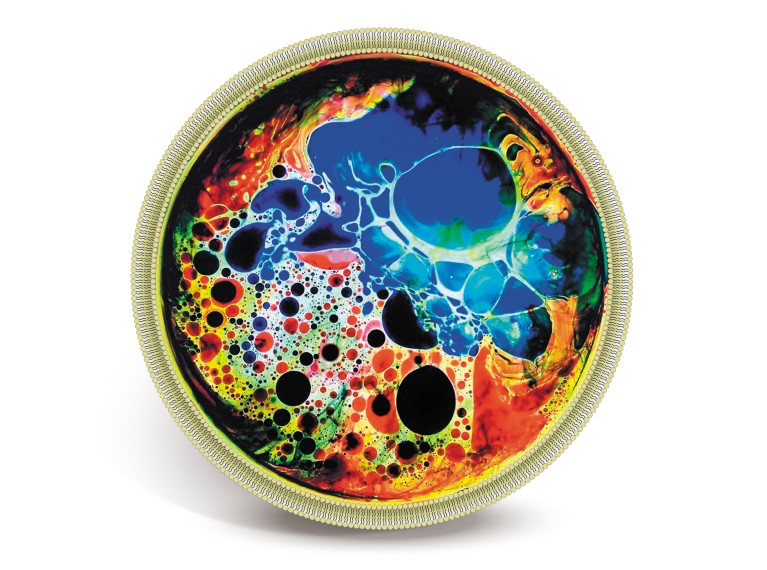
\includegraphics[width=\RightPanel]{representative-image.png}\\[\vskipSection] % name of the image 
\parbox{\RightPanel}{%
\fontsize{\CaptionSize}{\CaptionSizeBaseline}\selectfont
\textbf{Fig.1}\quad 
% 
% Title of the image (bold)
\textbf{Figure caption title.} 
% 
% Body of the image caption.
Figure caption text (body). Write something that completes/explains the figure and relates to the abstract.
%
% Credits.
\textit{Figure credits.} 
}
\end{tabular}
}% end right column

\end{tabular}
\end{document}
